\documentclass[12pt,a4paper]{article}
\usepackage{graphicx}
\usepackage{float}
\usepackage{tikz}
\usetikzlibrary{shapes, arrows, positioning, calc}


\usepackage{amsmath,amssymb,mdframed}   % AMS package gives better equation layouts
\setcounter{page}{2}                    % sets first page number to 2
\setlength{\oddsidemargin}{-0.25in}     % set left margin
\setlength{\textwidth}{6.5in}           % set text width
\setlength{\topmargin}{-0.5in}          % controls layout at
\setlength{\headsep}{0.5in}             % top of page
\setlength{\textheight}{9.0in}          % set text length



\makeatletter
\renewcommand{\@oddhead}{\hfill MA3604/19}  % sets header % TODO fix header
\renewcommand{\@oddfoot}{\hfil \arabic{page} \hfil}    % sets page footer
\makeatother

\renewcommand{\labelenumi}{\arabic{enumi}} % Sets the first level of enumerate to be arabic (normal) numbers
\renewcommand{\labelenumii}{(\alph{enumii})} %Sets the second level of enumerate to be (a), (b), (c), .....
\renewcommand{\labelenumiii}{(\roman{enumiii})} % Sets the third level of enumerate to be (i), (ii), (iii), ....



\begin{document}
\null \vskip1cm
\begin{enumerate}

\renewcommand\labelenumi{\bfseries\theenumi.}

\item

    \begin{enumerate}
        \item Give the definition of a normal form game.
        ~\hfill{[2]}
        \item Consider the normal form game with
            the following matrix representation:
            $$A=
                \begin{pmatrix}
                    30 & 6\\
                    12 & 30
                \end{pmatrix}
              \qquad
              B=
                \begin{pmatrix}
                    12 & 30\\
                    42 & 12
                \end{pmatrix}
            $$

            Consider the mixed strategies for the row player
            \(\sigma_r=(x,1-x)\) and the column player \(\sigma_c=(y,1-y)\).
            Sketch a plot of:

            \begin{itemize}
                \item the row player's utilities: \(u_r((1, 0), \sigma_c)\)
                    and \(u_r((0, 1), \sigma_c)\).
                    ~\hfill{[1]}
                \item the column player's utilities: \(u_c(\sigma_r, (1, 0))\)
                    and \(u_c(\sigma_r, (0, 1))\).
                    ~\hfill{[1]}
            \end{itemize}

            Using the plot, obtain the best responses of both
            players.~\hfill{[1]}

        \item Consider a modification of the above game where a third strategy
            is given to the column player:

            $$A=
                \begin{pmatrix}
                    30 & 6 & 36\\
                    12 & 30 & 18
                \end{pmatrix}
              \qquad
              B=
                \begin{pmatrix}
                    12 & 30 & 22\\
                    42 & 12 & 6
                \end{pmatrix}
            $$

            Sketch a plot of \(u_c(\sigma_r, (0, 0, 1))\).~\hfill{[2]}

            Using this plot and the plots of part (b) above, obtain the best
            responses for both players for this modified game.~\hfill{[4]}

        \item Give the definition of the row/column best response polytopes for
            a 2 player game \((A, B)\in\mathbb{R}^{{m\times n}^2}\).~\hfill{[2]}

        \item State the Lemke-Howson algorithm.
              ~\hfill{[4]}

        \item Using Tableaux, carry out the Lemke-Howson algorithm on the
            modified game. Describe how this confirms your finding of part
            (c)~\hfill{[8]}
    \end{enumerate}

\newpage
\item

    \begin{enumerate}
        \item Give the definition of a repeated game.
            ~\hfill{[2]}
        \item Give the definition of strategy in a repeated game.
            ~\hfill{[2]}

        \item Consider the following stage
            game:

            \[
                A = \begin{pmatrix}
                    1 & 4 & -1\\
                    -1 & 0 & -2\\
                    \end{pmatrix}
                \qquad
                B = \begin{pmatrix}
                    -2 & 5 & 5\\
                    18 & -1 & -2\\
                    \end{pmatrix}
            \]


            Obtain all possible histories for the corresponding 2 stage repeated
            game.
            ~\hfill{[3]}

        \item Obtain all Nash equilibria for the 2 stage repeated game of
            part (c)
            that are sequences
            of stage Nash equilibria.
            ~\hfill{[4]}

        \item Obtain a Nash equilibrium that is not a sequence of stage Nash
            equilibria for the 2 stage repeated game of part (c). Justify
            this.
            ~\hfill{[5]}

        \item Consider the Centipede game which can be represented by the
            following diagram:

            \begin{center}
                \begin{tikzpicture}[scale=.8, every node/.style={scale=0.8}]

                    \node [draw] (A) at (0, 0) {(A: P1)};
                    \node [draw] (Astop) at ($(A) - (0, 2)$) {(2, 0)};
                    \node [draw] (B) at ($(A) + (4, 0)$) {B: P2};
                    \node [draw] (Bstop) at ($(B) - (0, 2)$) {(1, 3)};
                    \node [draw] (C) at ($(B) + (4, 0)$) {C: P1};
                    \node [draw] (Cstop) at ($(C) - (0, 2)$) {(4, 2)};
                    \node [draw] (D) at ($(C) + (4, 0)$) {D: P2};
                    \node [draw] (Dstop) at ($(D) - (0, 2)$) {(3, 5)};
                    \node [draw] (Dcontinue) at ($(D) + (4, 0)$) {(4, 4)};

                    \draw [->] (A) -- node [above] {Continue} (B);
                    \draw [->] (B) -- node [above] {Continue} (C);
                    \draw [->] (C) -- node [above] {Continue} (D);
                    \draw [->] (D) -- node [above] {Continue} (Dcontinue);

                    \draw [->] (A) -- node [left] {Stop} (Astop);
                    \draw [->] (B) -- node [left] {Stop} (Bstop);
                    \draw [->] (C) -- node [left] {Stop} (Cstop);
                    \draw [->] (D) -- node [left] {Stop} (Dstop);
                \end{tikzpicture}
            \end{center}

            Players take turns:

            \begin{itemize}
                \item At step (A), the first player can choose to stop
            in which case they get a utility of 2 and the second player a
            utility of 0.
                \item If the first player chooses to continue, then at step (B), the
            second player can choose to stop in which case they get a utility of
            3 and the first player a utility of 1.
                \item If the second player chooses to continue,
            then at step (C), the first player can choose to stop in which case
            they get a utility of 4 and the second player a utility of 2.
                \item If the first player choose to continue, then at step (D),
                    the second player can choose to stop in which case they get
                    a utility of 5 and the first player a utility of 3.
                \item If the second player chooses to continue then both players
                    get a utility of 4.
            \end{itemize}

            Show how this game can also be represented as a Normal form game
            with the following matrices:

                \[A =
                         \begin{pmatrix}
                             4 & 3 & 1 & 1\\
                             4 & 4 & 1 & 1\\
                             2 & 2 & 2 & 2\\
                             2 & 2 & 2 & 2\\
                         \end{pmatrix}
                         \qquad
                         B =
                         \begin{pmatrix}
                             4 & 5 & 3 & 3\\
                             2 & 2 & 3 & 3\\
                             0 & 0 & 0 & 0\\
                             0 & 0 & 0 & 0\\
                         \end{pmatrix}
                  \]

            ~\hfill{[6]}


      \item Obtain the Nash equilibria in pure strategies for the Centipede game
          described in part (f). ~\hfill{[3]}

    \end{enumerate}

\newpage
\item

    \begin{enumerate}
        \item Give the general definition of the Prisoner's Dilemma.
            ~\hfill{[2]}
        \item What values of $S, T$, if any, give valid Prisoner's Dilemma games
            for:
            \begin{enumerate}
                \item  \(A =
                         \begin{pmatrix}
                            3 & S\\
                            6 & 1
                         \end{pmatrix}
                         \qquad
                         B =
                         \begin{pmatrix}
                            3 & T\\
                            -1 & 1
                         \end{pmatrix}
                       \)
                ~\hfill{[4]}
                \item  \(A =
                         \begin{pmatrix}
                            2 & S\\
                            -2 & 1
                         \end{pmatrix}
                         \qquad
                         B =
                         \begin{pmatrix}
                            2 & -2\\
                            S & 1
                         \end{pmatrix}
                       \)
                ~\hfill{[4]}
            \end{enumerate}
        \item For the remainder of this question, consider the following game:
            \[A =
                         \begin{pmatrix}
                            b - c & c\\
                            b & 1
                         \end{pmatrix}
                         \qquad
                         B =
                         \begin{pmatrix}
                             b - c & b\\
                             c & 1
                         \end{pmatrix}
                     \]
                What conditions need to hold on \(b, c\) to ensure that the game
                is a Prisoners Dilemma?
                ~\hfill{[5]}
         \item Consider two reactive players \(p=(p_1, p_2)\) and \(q=(q_1,
             q_2)\). Stating any results you use show that the expected utility
             for player \(p\) is given by:

             $$s_1s_2\times (b - c) +  s1(1-s_2) \times c +  (1-s_1)s_2 \times b +
            (1-s_1)(1-s_2)$$

             where:

             $$
             s_1 = \frac{q_2r_1+p_2}{1-r_1r_2}\qquad s_2 =
             \frac{p_2r_2+q_2}{1-r_1r_2}
             $$

             for:

             $$r_1=p_1-p_2\qquad r_2=q_1-q_2$$

             ~\hfill{[3]}

         \item Using this, for \((b, c) = (2, 1/2)\), show that the utility of
             the first player is given by:
             ~\hfill{[3]}

             \[
                 s_2 - s_1/2 + 1
             \]

         \item What is the optimal behaviour against a player \(q\) for which
             \(q_1=q_2\)?
             ~\hfill{[4]}
    \end{enumerate}
\newpage
\item

    \begin{enumerate}
        \item For a matrix \(A=\begin{pmatrix}a&b\\c &d\end{pmatrix}\), obtain
              the following equation describing the corresponding evolutionary
              game:
              \[\frac{dx}{dt}=x(f-\phi)\]
              where \(f=Ax\) and \(\phi=fx\).
              ~\hfill{[2]}
        \item Define a mutated population.
              ~\hfill{[2]}
        \item Define an evolutionary stable strategy.
              ~\hfill{[2]}
        \item State and prove a theorem giving a general condition for an
            evolutionary stable strategy.
              ~\hfill{[4]}
        \item Consider the following game
        \(A=\begin{pmatrix}2&3\\0 &1\end{pmatrix}\). Obtain all evolutionary
            stable strategies.
              ~\hfill{[5]}
         \item Consider the accompanying 2008 paper entitled ``Studying the
             emergence of invasiveness in tumours using game theory'' by Basanta
             et al.
             \begin{enumerate}
                 \item Give a general summary of the paper.
                     ~\hfill{[3]}
                 \item There is a minor error in this paper in the game matrix.
                     Describe and suggest the fix.~\hfill{[2]}
                 \item How does the theorem in part (d) of this question relate to
                     the findings of the paper?~\hfill{[2]}
                 \item Suggest an alternative area of game theory that could
                     also be used.~\hfill{[3]}
             \end{enumerate}
     \end{enumerate}
 \end{enumerate}

\makeatletter
\renewcommand{\@oddfoot}{\hfil \arabic{page}X \hfil}    % sets last page footer
\makeatother

\end{document}
